\documentclass[a4paper, 11pt]{report}

\usepackage{a4wide,cite}
\usepackage[utf8]{inputenc}
\usepackage{amsmath, amsthm, amssymb, units, dsfont, algorithmicx, algpseudocode, nomencl}   % dsfont pro indikátor jevu
\usepackage[pdftex,
						pdfauthor={Jakub Klemsa},
						pdftitle={Models of self-assembling DNA nanostructures, Jakub Klemsa},
						pdfsubject={},
						pdfkeywords={Wang tiles, aTAM, Turing universality},
						pdfproducer={Jakub Klemsa},
						pdfcreator=dvipdf]{hyperref}
\usepackage{graphicx,color,tabularx,float}
\usepackage{fancyhdr}
\pagestyle{fancy}
\fancyhf{}
\fancyhead[L]{\slshape \rightmark} % \leftmark .. kapitola
\fancyhead[R]{\thepage}
\oddsidemargin=10mm   % jednostranný tisk !!!
\makenomenclature   % vyrobí nomenklaturu

\let\tmpitem\item
\renewcommand{\item}{\setlength{\itemsep}{2pt}\tmpitem}   % míň roztahovačný seznamy
\renewcommand{\labelitemi}{$\circ$}
%~ \def\refname{Li­teratura}   % záhadně nefunguje ???
%~ \frenchspacing   % údajně česká typografická pravidla

\theoremstyle{definition}
\newtheorem{example}{Example}[chapter]
%~ \newtheorem{definition}{Definice}[section]
%~ \newtheorem{predpoklad}{Předpoklad}[section]
%~ \newtheorem{tvrzeni}{Tvrzení}[section]
%~ \newtheorem{pozorovani}[tvrzeni]{Pozorování}
%~ \newtheorem{lemma}[tvrzeni]{Lemma}
%~ \newtheorem{dusledek}[tvrzeni]{Důsledek}
%~ \newtheorem{algoritmus}{Algoritmus}[chapter]

%~ \theoremstyle{remark} 
%~ \newtheorem{pozn}{Poznámka}[chapter]

\DeclareMathOperator*{\E}{E\,}   % operátor* bude umět používat \limit :)
\DeclareMathOperator{\de}{d\!}   % v integrálech
\renewcommand{\P}{\mathbb{P\,}}
\newcommand{\R}{\mathbb{R}}
\newcommand{\Z}{\mathbb{Z}}
\newcommand{\N}{\mathbb{N}}
\newcommand{\indicator}{\mathds{1}}
\newcommand{\powerset}[1]{\mathcal{P} ( #1 )}
\newcommand{\adob}[2]{#1 , \ldots , #2}

%%% VYHLEDAT A OPRAVIT !!! %%%%%%%%%%%%%%%%%%%%%%%%%%%%%%%%%%%%%%%%%%%%%
\let\haluz\relax
\let\hobza\relax
\haluz % program vlna nakonec!
% naučit se psát jednoduchý konsekventy! viz Adleman str. 3 nahoře: "Note that the labeling ..."
% taky opravit N-1 na N\!-\!1
% zkontrolovat \min \; ...
%%%%%%%%%%%%%%%%%%%%%%%%%%%%%%%%%%%%%%%%%%%%%%%%%%%%%%%%%%%%%%%%%%%%%%%%

%%% k vyplnění ZAČÁTEK -------------------------------------------------
\newcommand{\cvut}{ČESKÉ VYSOKÉ UČENÍ TECHNICKÉ V~PRAZE}
\newcommand{\fjfi}{Fakulta jaderná a fyzikálně inženýrská}
\newcommand{\km}{Katedra matematiky}
\newcommand{\obor}{Inženýrská informatika}
\newcommand{\minf}{Matematická informatika}
\newcommand{\TYPPRACE}{VÝZKUMNÝ ÚKOL}
\newcommand{\TypPrace}{Výzkumný úkol}
\newcommand{\mePrace}{mého výzkumného úkolu}
\newcommand{\rodPrace}{ho}

\newcommand{\nazevcz}{Modely sebeskládajících DNA nanostruktur}
\newcommand{\nazeven}{Models of self-assembling DNA nanostructures}
\newcommand{\autor}{Jakub Klemsa}
\newcommand{\vedouci}{Ing. Štěpán Starosta, Ph.D.}
\newcommand{\vedoucimu}{Ing. Štěpánu Starostovi, Ph.D.}
\newcommand{\pracovisteVed}{}
\newcommand{\konzultant}{---}
\newcommand{\rok}{2014}
\newcommand{\akadRok}{2013/2014}
\newcommand{\misto}{Praha}
\newcommand{\vMiste}{Praze}

\newcommand{\klicova}{Klíčová.}
\newcommand{\keyword}{Keywords.}
\newcommand{\abstrCZ}{Abstrakt CZ.}
\newcommand{\abstrEN}{Abstrakt EN.}
%%% k vyplnění KONEC ---------------------------------------------------


\begin{document}


\pagenumbering{roman}
\begin{titlepage}

%%% 1. úvodní strana
\thispagestyle{empty}
\begin{center}
	{\Large \cvut \\[12pt] \fjfi \\[260pt]}
	{\Huge \TYPPRACE}
\end{center}
\vfill
{
	\Large \misto, \rok \hfill \autor
}
\newpage


%%% 2. úvodní strana
\thispagestyle{empty}
\begin{center}
	{\Large \cvut \\[10pt] \fjfi \\[10pt] \km \\[40pt]}
	
\includegraphics[height=75pt]{lev.pdf} \\[100pt]
	
	{\LARGE \TYPPRACE \\[60pt]}
	
	{\Large\bf \nazevcz \\[30pt]}
	
	{\Large\bf \nazeven}
\end{center}
\vfill
{
	\Large
	\begin{tabular}{ll}
	Vypracoval: & \autor\\[3pt]
	Školitel: & \vedouci\\[3pt]
	Akademický rok: & \akadRok
	\end{tabular}
}
\newpage


%%% sem přijde ofic. zadání
\thispagestyle{empty}
\Large
Na toto místo přijde svázat \textbf{zadání \mePrace}!

\vspace{4mm}
V~jednom z~výtisků musí být \textbf{originál} zadání, v~ostatních kopie.
\normalsize
\newpage


%%% prohlášení
\thispagestyle{empty}
~
\vfill
\noindent\textbf{Čestné prohlášení}
\vspace{0.5cm}

\noindent
Prohlašuji na tomto místě, že jsem předloženou práci vypracoval samostatně a že jsem uvedl veškerou použitou literaturu.
\vspace{1.5cm}

\noindent
\vspace{5mm}V \vMiste ~dne \today\hfill
	\begin{tabular}{c}
	. . . . . . . . . . . . . . . . . . . . . . .\\
	\autor
	\end{tabular}
\newpage


%%% poděkování
\thispagestyle{empty}
~
\vfill
\noindent\textbf{Poděkování}
\vspace{0.5cm}

\noindent
Děkuji \vedoucimu, za vedení \mePrace ~a za podnětné návrhy, které \rodPrace ~obohatily.

\begin{flushright}
\autor
\end{flushright}
\newpage


%%% abstrakt atp.
\thispagestyle{empty}

\begin{tabularx}{\textwidth}{lX}
  {\em Název práce:} & \bf \nazevcz \\[4mm]
  {\em Autor:} & \autor \\[4mm]
  {\em Obor:} & \obor \\[4mm]
  {\em Zaměření:} & \minf \\[4mm]
  {\em Druh práce:} & \TypPrace \\[4mm]
  {\em Vedoucí práce:} & \vedouci, \pracovisteVed \\[4mm]
  {\em Konzultant:} & \konzultant \\[4mm]
  {\em Abstrakt:} & \abstrCZ \\[4mm]
  {\em Klíčová slova:} & \klicova \\[20mm]

  {\em Title:} & \bf \nazeven \\[4mm]
  {\em Author:} & \autor \\[4mm]
  {\em Abstract:} & \abstrEN \\[4mm]
  {\em Key words:} & \keyword
\end{tabularx}
\newpage


%%% nomenklatura \haluz nefunguje
\thispagestyle{empty}
\printnomenclature
\newpage


%%% obsah
\tableofcontents
\thispagestyle{empty}

\end{titlepage}
\pagenumbering{arabic}


%%%%%%%%%%%%%%%%%%%%%%%%%%%%%%%%%%%%%%%%%%%%%%%%%%%%%%%%%%%%%%%%%%%%%%%%
%     Z A Č Á T E K   P R Á C E                                        %
%%%%%%%%%%%%%%%%%%%%%%%%%%%%%%%%%%%%%%%%%%%%%%%%%%%%%%%%%%%%%%%%%%%%%%%%


%%% ÚVODEM
\cleardoublepage\phantomsection   % cleardoublepage a phantomsection udělají že odkaz z obsahu vede NAD nadpis, jinak vede POD
\addcontentsline{toc}{chapter}{Prolog}
\chapter*{Prolog}

	1959: Feynman's visionary talk, \cite{feynman}; 
	
	The ground-breaking work was carried out by Adleman, \cite{adleman94}, who showed that DNA computation is practically feasible. In his experiment, Adleman used special DNA sequences for solving Hamiltonian Path Problem, one of the most typical NP-complete problems.
	
	... Extreme parallelism! But also possibility of errors.

\section*{Work overview}
	
	%%%%%%%%%%%%%%%%%%%%%%%%%%%%%%%%%%%%%%%%%%%%%%%%%%%%%%%%%%%%%%%%%%%%%%
	
	Chapter 1: Intro.\\
	Chapter 2: First of all I will describe models which exploit specific DNA structure.\\
	Chapter 3: Abstract Tile Assembly Model, temperature, 2D vs. 3D.\\
	Positive integers $\N$. \nomenclature{$\N$}{Positive integers.}
	
	% zkusíme Ramseyovo číslo R(5,5) ? :)
	% -> problém "Je R(n,n) větší než něco?" znamená pro odpověď ANO najít graf t.ž. neobsahuje K_n ani anti-K_n .. což je samo o sobě co-NP (neboli to je \exists \forall stroj .. \Sigma_2 jazyk, horní hranice pak je \Pi_2 jazyk)
	% 
	% NP vs co-NP .. co-NP přece nedává ne?

%%% KAPITOLA 1
\chapter{Introduction to DNA computation}
\label{chap:intro}

	
	1959: Feynman's visionary talk, \cite{feynman}; pros: extreme paralelism, cons: reliability.
	
	The ground-breaking work was carried out by Adleman, \cite{adleman94}, who showed that DNA computation is practically feasible. In his experiment, Adleman used special DNA sequences for solving Hamiltonian Path Problem, one of the most typical NP-complete problems.
	
	... Extreme parallelism! But also possibility of errors.

\section*{Work overview}
	
	%%%%%%%%%%%%%%%%%%%%%%%%%%%%%%%%%%%%%%%%%%%%%%%%%%%%%%%%%%%%%%%%%%%%%%
	
	Chapter 1: Intro.\\
	Chapter 2: First of all we will describe models which exploit specific DNA structure.\\
	Chapter 3: Abstract Tile Assembly Model, temperature, 2D vs. 3D.\\
	Positive integers $\N$. \nomenclature{$\N$}{Positive integers.}
	
	% zkusíme Ramseyovo číslo R(5,5) ? :)
	% -> problém "Je R(n,n) větší než něco?" znamená pro odpověď ANO najít graf t.ž. neobsahuje K_n ani anti-K_n .. což je samo o sobě co-NP (neboli to je \exists \forall stroj .. \Sigma_2 jazyk, horní hranice pak je \Pi_2 jazyk)
	% 
	% NP vs co-NP .. co-NP přece nedává ne?

\section{Basic DNA principles}
	
	DNA (deoxyribonucleic acid) is a large biomolecule carrying living organisms' genetic information. Its most common structure is well known double-helix which consists of two strands connected by hydrogen bonds. These strands are biopolymers built up by {\em polymerase chain reaction} (PCR) from small units -- nucleotides. Each nucleotide consists of two parts: nitrogenous base and backbone molecules.
	\begin{description}
		\item[Nitrogenous bases] There are $4$ nucleobases in DNA ($+1$ in RNA): Adenine ({\bf A}), Thymine ({\bf T}), Cytosine ({\bf C}), Guanine ({\bf G}) and Uracil ({\bf U}) in RNA instead of Thymine in DNA. These molecules are responsible for making hydrogen bonds between strands in a manner following Watson-Crick complementarity: only {\bf A} -- {\bf T} and {\bf C} -- {\bf G} pairs can be formed.
		\item[Backbone molecules] Backbone of DNA strand is made of alternating deoxyriboses and phosphates. Phosphates only hold adjacent deoxyriboses, each deoxyribose moreover holds one nucleobase. Due to deoxyribose carbon numbering, DNA backbone has so called $5'$ and $3'$ ends, default reading order is $5'\rightarrow 3'$. DNA strands must be antiparallel so that nucleobases can connect.
	\end{description}

\section{Complexity, languages}
	
	\subsection{$O$ and other notations}
		
		Let us briefly remind $O$-, $o$-, $\Omega$-, $\omega$- and $\Theta$-notations for $f, g: \N \rightarrow \N$. We will denote $(\exists n_0 \in \N) (\forall n > n_0)$ shortly by $(\forall^* n)$ which can be read ``for almost all $n$''. Also $(\forall n_0 \in \N) (\exists n > n_0)$ will be denoted by $(\exists^\infty n)$ which can be read ``there exist infinitedly many $n$''.
		\begin{defn}
		\begin{align*}
			g \in O(f) &\iff (\exists C > 0) (\forall^* n) \bigl(g(n) < C f(n)\bigr) \\[5pt]
			g \in \omega^{(1)}(f) &\iff (\forall C > 0) (\exists^\infty n) \bigl(g(n) > C f(n)\bigr) \\[5pt]
			g \in \omega^{(2)}(f) &\iff (\forall C > 0) (\forall^* n) \bigl(g(n) > C f(n)\bigr) \\[5pt]
			g \in \Omega^{(1)}(f) &\iff (\exists C > 0) (\exists^\infty n) \bigl(g(n) > C f(n)\bigr) \\[5pt]
			g \in \Omega^{(2)}(f) &\iff (\exists C > 0) (\forall^* n) \bigl(g(n) > C f(n)\bigr) \\[5pt]
			g \in o(f) &\iff (\forall C > 0) (\forall^* n) \bigl(g(n) < C f(n)\bigr) \\[5pt]
			g \in \Theta(f) &\iff (\exists C_1, C_2 > 0) (\forall^* n) \bigl(C_1 f(n) \leq g(n) \leq C_2 f(n)\bigr) \\[5pt]
			g \sim f &\iff \lim\limits_{n\to\infty} \frac{g(n)}{f(n)} = 1
		\end{align*}
		\end{defn}
		
		\begin{remark}
			Note that there are two different definitions for omegas. $\Omega^{(1)}$ is equivalent to the orgininal definition introduced by Hardy \cite{hardy1914} which states
			\begin{equation}
				f \in \Omega(g) \iff \limsup\limits_{n\to\infty}\frac{f(n)}{g(n)} > 0 .
			\end{equation}
			The other, $\Omega^{(2)}$, was introduced by Knuth from good reasons described in \cite{knuth76}. In similar manner there are two definitions for $\omega$.
			
			Note that there are also some relations: the condition for $\Omega^{(1)}$ is negation of the condition for $o$ so these sets are complementary for given function $f$, similarly for $\omega^{(1)}$ and $O$. For the second variant one can easily check that $f\in\Omega^{(2)}(g)\iff g\in O(f)$ and $f\in\omega^{(2)}(g)\iff g\in o(f)$. There is also an equivalent condition for $\Theta$:
			\begin{equation}
				g \in \Theta(f) \iff g \in O(f) \,\wedge\, f \in O(g) \iff g \in O(f) \,\wedge\, g \in \Omega^{(2)}(f) .
			\end{equation}
			
			The condition for $g \sim f$ can be easily seen to be equivalent to $|f-g| \in o(g)$. In chapter~\ref{chap:problems} we will be mostly interested in this relation because it specifies the function better than $\Theta$. For example, $2n \in \Theta(n)$ but $2n \not\sim n$.
		\end{remark}
	
	\subsection{Studied complexities}
		
		\begin{defn}
			All the following complexities are considered as functions of input length:
			{\em Biostep complexity} will refer to the number of laboratory steps needed to handle the computation. Winfree \cite{winfree_phd} describes formally few types of such lab procedures for operations with Boolean strings ({\em Separate[i], Merge, Detect, Amplify and Append}), Adleman \cite{adleman94} describes couple of them more practically.\\
			{\em Tile complexity} will refer to the number of different DNA tiles needed.\\
			{\em Glue complexity} will refer to the number of different sticky-end sequences needed (commonly referred to as {\em glues}). Each sequence with its Watson-Crick complement is considered as only one glue.
		\end{defn}
	
	\subsection{Languages}
		
		\begin{defn}
			Let $\Sigma$ be an nonempty finite set of {\em characters} which will be referred to as {\em alphabet}. Define set of {\em words} over alphabet $\Sigma$ as $\Sigma^* = \bigcup_{n\in\N_0}\Sigma^n$ and set of nonempty words as $\Sigma^+ = \bigcup_{n\in\N}\Sigma^n$. Empty word will be denoted by $\varepsilon$. {\em Language} ${\cal L}$ over alphabet $\Sigma$ is then just a set of words: ${\cal L} \subseteq \Sigma^*$.
		\end{defn}
		
		What is a formal language? Regular, context-free and recursively enumerable languages.
		% is equivalent to boolean functions over \N
	
	\subsection{P, NP and other classes}
		
		First two definitions are from \cite{book_comp}.
		
		\begin{defn}
			${\cal L} \subseteq \Sigma^*$. ${\cal L} \in NP \iff \bigl(\exists p, q \in {\cal P}\bigr) \bigl(\exists \textnormal{ deterministic Turing machine } M\bigr)\\ \bigl(\forall x \in \Sigma^*\bigr) \Bigl(x \in {\cal L} \iff \bigl(\exists y \in \Sigma^{p(|x|)}\bigr) \bigl(M \textnormal{ accepts } (x,y) \textnormal{ in time } \leq q(|x|+|u|)\bigr)\Bigr)$.\\
			Such $y$ will be referred to as {\em certificate} for $x$ (with respect to $\cal L$ and $M$).
		\end{defn}
		
		\begin{defn}
			${\cal L} \subseteq \Sigma^*$. ${\cal L} \in co\textnormal{-}NP \iff \bigl(\exists p, q \in {\cal P}\bigr) \bigl(\exists \textnormal{ deterministic Turing machine } M\bigr)\\ \bigl(\forall x \in \Sigma^*\bigr) \Bigl(x \in {\cal L} \iff \bigl(\forall y \in \Sigma^{p(|x|)}\bigr) \bigl(M \textnormal{ accepts } (x,y) \textnormal{ in time } \leq q(|x|+|u|)\bigr)\Bigr)$.
		\end{defn}
		
		\begin{defn}
			$DTime\bigl(f(n)\bigr) = \bigl\{ {\cal L}\textnormal{ language} \bigm| (\exists \textnormal{ deterministic Turing machine }M)\\ \bigl(x\in{\cal L} \iff M\textnormal{ accepts }x\textnormal{ in time }\leq f(|x|)\bigr) \bigr\}$.\\
			Other classes are defined in a very similar manner (time $\leftrightarrow$ space, deterministic $\leftrightarrow$ non-deterministic).
		\end{defn}
		\noindent
		Now we can easily define well-known classes $P$ and $NP$.
		\begin{defn}
			$P = \bigcup\limits_{k\in\N} DTime(n^k)$ and $NP = \bigcup\limits_{k\in\N} NTime(n^k)$.
		\end{defn}
		
		
		
	\begin{center}\line(1,0){400}\end{center}
	Biostep complexity, tile complexity, glue complexity.
	
	P, NP, co-NP, PP, \#P, PSpace. Enough? Maybe also polynomial hierarchy: $\Sigma_k P$ and $\Pi_k P$ languages (alternating Turing machine with bounded alternation, \cite{kozen06}).
	
	% $ \textnormal{NP} = \bigl\{ L \subseteq \Sigma^* \bigm| \exists p_{1,2} \in \mathcal{P} \; \forall x \in L \; \exists y \in L \bigl( |y| \leq p_1(|x|) \,\wedge\, R(x,y) \textnormal{ s.t. R is enumerable in time } \leq p_2(|x|+|y|) \bigr) \bigr\} $
	
	Regular languages, context-free languages, recursively enumerable languages.
	
	%%%%%%%%%%%%%%%%%%%%%%%%%%%%%%%%%%%%%%%%%%%%%%%%%%%%%%%%%%%%%%%%%%%%%%
	
	HPP: Adleman uses $O(n)$ biosteps, Winfree one.
	SAT: Lipton's contribution using $m$ biosteps ($m = \#clauses$), \cite{lipton95}, Lipton's set of speedup problems, \cite{lipton96speedup}.
	Lipton 95 describes basic DNA operations.
	Energy efficiency (Adleman).
	NP definition?

\section{Strand models}
	
	There exist or can be synthesized many types of molecules, well described in Winfree \cite{winfree_comp} even with their inception reaction. The most important structures are linear strands (Sections \ref{sec:lin_strands}, \ref{sec:adleman}, Figure \ref{fig:linear}), dendrimer structures (Section \ref{sec:dendrimer}, Figure \ref{fig:dendrimer}) and double crossover molecules (Section \ref{sec:double_crossover}, Figure \ref{fig:double_crossover}).
	\begin{note}\label{note:untwist}
		DNA naturally forms double-helices which would be confusing in figures so there will mostly appear schemes of ``untwisted'' molecules, only double crossover molecules will be described more precisely. % nebo snad unscrewed?
	\end{note}
	
	\subsection{Linear strands}
	\label{sec:lin_strands}
		
		Linear strands are just a piece of double-helix with two types of ends: either with one strand longer than the other (sticky end) or with both strands connected to each other. The top molecule in Figure \ref{fig:linear} is called {\em hairpin}.
		\begin{figure}[h]
		\begin{center}
			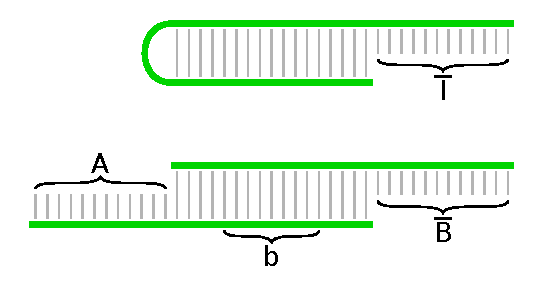
\includegraphics[width=0.502\textwidth]{./figures/strand_types/linear.pdf} % {šířka v mm}/370 je to původně
			\caption{Linear strands: a strand for initial symbol $I$ and a strand for rule $A\rightarrow bB$.}
			\label{fig:linear}
		\end{center}
		\end{figure}
		Winfree \cite{winfree_phd} proved that restricted class of linear strands is equivalent to regular languages, this means
		\begin{itemize}
			\item given a set of linear strands, the generated language is regular,
			\item given a regular language there exists a set of linear strands which generate it.
		\end{itemize}
		Figure \ref{fig:linear} shows how to assign grammar rules to linear strands.
	
	\subsection{Adleman's experiment}
	\label{sec:adleman}
		
		Linear strands were used in Adleman's ground-breaking work \cite{adleman94}. He showed that DNA molecules are really capable of computation. He exploited the huge parallelism in DNA computation for one of the most fundamental $\NPC$ problems -- the Hamiltonian Path Problem ($\sf HPP$) in directed graph with designated vertices $v_{begin}$ and $v_{end}$.
		
		Let us remind this type of $\sf HPP$. Given a directed graph $G_n$ with $n$ vertices and two designated vertices $v_{begin}$ and $v_{end}$, the problem is to answer whether there exists an oriented path from $v_{begin}$ to $v_{end}$ through the graph such that the path visits every vertex. Note that {\em path} cannot visit any vertex more than once from definition.
		
		\begin{figure}[h]
		\begin{center}
			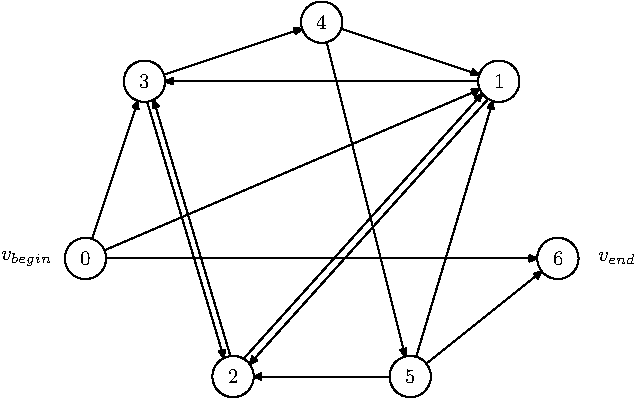
\includegraphics{./figures/adleman_graph.pdf}
			\caption{Adleman's original graph.}
			\label{fig:adleman_graph}
		\end{center}
		\end{figure}
		
		Adleman originally used a graph with seven vertices shown in Figure \ref{fig:adleman_graph}. It can be seen that the path $0 \rightarrow 1 \rightarrow 2 \rightarrow 3 \rightarrow 4 \rightarrow 5 \rightarrow 6$ is Hamiltonian\footnote{Note that it can be re-labelled in such a nice way without loss of generality.}.
		
		Adleman first presented the following non-deterministic five-step algorithm, whose steps were described in his work in terms of DNA manipulations:
		\begin{description}
			\item[Step 1.] Generate random paths through the graph.
			\item[Step 2.] Keep only those paths that begin with $v_{begin}$ and end with $v_{end}$.
			\item[Step 3.] If the graph has $n$ vertices, then keep only those paths that enter exactly $n$ vertices.
			\item[Step 4.] Keep only those paths that enter all of the vertices of the graph at least once.
			\item[Step 5.] If any path remains, say ``Yes''; otherwise, say ``No.''\footnote{This is the original version, I would rectify the fifth step: If any paths remain, say ``Yes''; otherwise say ``{\em I do not know}''. That is because it may happen that there exists a valid path but unfortunately it did not assemble or got lost. Note the similarity to $\NP$ versus $\coNP$, see Section \ref{sec:PNP}.} %!% citaci, někdo to už taky kritizoval
		\end{description}
		To see % sloveso od insight ?
		how DNA can compute, let us describe this example more precisely. The computation itself (meaning the inception of the final solution) is hidden in Step 1. Each vertex $i$ is associated with a random\footnote{We will expect those sequences to be different enough.} $20$-mer sequence of DNA, let us denote its $5'\rightarrow 3'$ orientation by $O_i$, its 10-mer prefix by $p_i$ and its 10-mer suffix by $q_i$. Each edge $i\rightarrow j$ is then associated with $O_{i\rightarrow j} = \overline{q_i p_j}$ sequence with reverse backbone orientation where $\overline{a}$ stands for Watson-Crick complementary word to the word $a$. There is an exception for $i=v_{begin}$, $j=v_{end}$ and every $k$: instead of $\overline{q_i p_k}$ there is $\overline{O_i p_k}$ and in a similar way for $j=v_{end}$.
		
		\begin{figure}[H]
		\begin{center}
			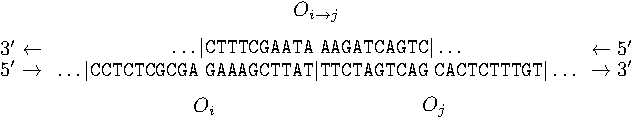
\includegraphics{./figures/adleman_strands.pdf}
			\caption{Example of assigned sequences.}
			\label{fig:adleman_strands}
		\end{center}
		\end{figure}
		
		It can be easily seen that all correctly bonded double-strands correspond with a valid walk through $G_n$. Moreover, all double-strands without sticky ends represent a valid walk from $v_{begin}$ to $v_{end}$ through $G_n$.
		
		All the other steps are fully described in \cite{adleman94}. The most important thing is that the most time-demanding step is Step 4. In this step one has to purify the product of Step 3 with a {\em biotin-avidin magnetic beads system}. This process consequently extracts for every vertex $i$ only those DNA strands which contain a substring representing vertex $i$. Thus this algorithm requires $O(n)$ laboratory steps which we will later consider unfeasible. Better solution with $O(1)$ laboratory steps was introduced by Winfree \cite{winfree_phd}.
	
	\subsection{Dendrimer structures}
	\label{sec:dendrimer}
		
		Dendrimer structures are multi-strand molecules which form such trees, see Figure \ref{fig:dendrimer}. There can be arbitrary\footnote{At this moment the model is theoretical though practically it has limitations. Note that even with limited number of branches the size of the whole system must be limited: having $O(2^n)$ molecules, they must fit in space $O(n^3)$ thus $n$ must be limited.} number of ends of both types, see Figure \ref{fig:linear}. Winfree \cite{winfree_phd} proved similar property as for linear strands: dendrimer structures are equivalent to context-free languages. Figure \ref{fig:dendrimer} shows an example of a context-free rule.
		
		\begin{figure}[h]
		\begin{center}
			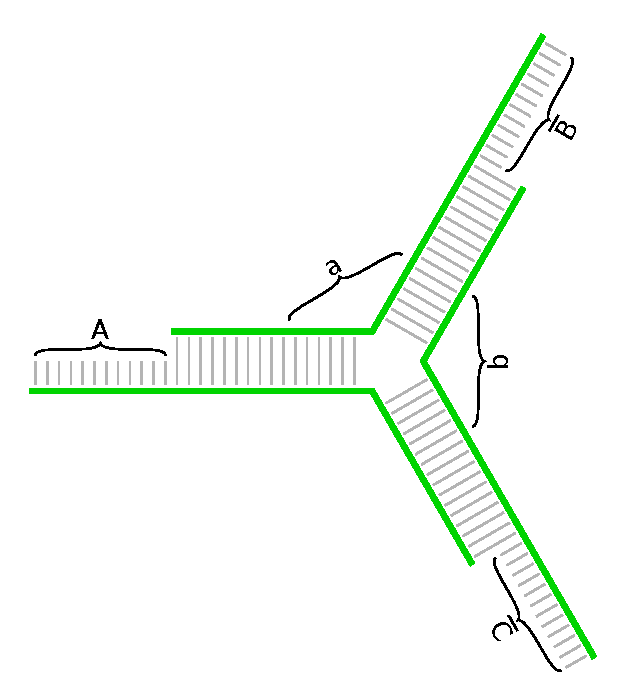
\includegraphics[width=0.568\textwidth]{./figures/strand_types/dendrimer.pdf}
			\caption{Dendrimer structure for rule $A\rightarrow aBbC$.}
			\label{fig:dendrimer}
		\end{center}
		\end{figure}
	
	\subsection{Double crossover molecules}
	\label{sec:double_crossover}
		
		Double crossover molecules are the most important ones. Though they are more complicated they are still very rigid, see \cite{seeman93}. Moreover they are theoretically capable of universal computation, see \cite{winfree_phd}. As we mentioned in Note \ref{note:untwist} we will also describe their inner structure. % universal computation: Winfree pg 57
		
		\begin{figure}[h]
		\begin{center}
			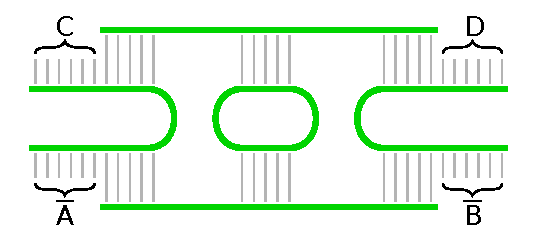
\includegraphics[width=0.492\textwidth]{./figures/strand_types/double_crossover.pdf}
			\caption{Double crossover molecule scheme.}
			\label{fig:double_crossover}
		\end{center}
		\end{figure}
		
		There are many possibilities how those strands can be twisted and connected. The most common ones are DAE and DAO molecules (Double-crossover, Antiparallel helical strands, Even or Odd, respectively, number of half-turns between crossovers), see Figure \ref{fig:dao-dae}. It can be seen that DAO molecules form tilings with strands jumping from one stage to another, on the other hand DAE molecules form tilings with a strand leading through entire stage in a row.
		
		\begin{figure}[h]
		\begin{center}
			\begin{subfigure}[b]{0.433\textwidth} % 130mm/300
				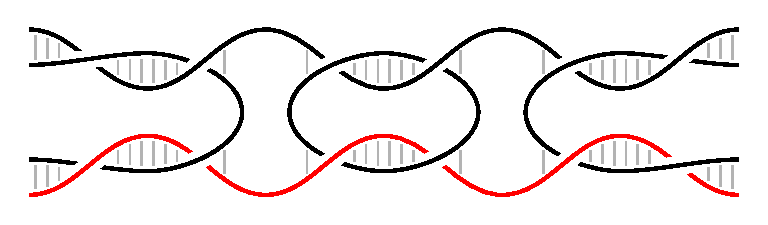
\includegraphics[width=\textwidth]{./figures/dao-dae/dae.pdf}
				\caption{DAE.}
				\label{fig:dao}
			\end{subfigure}
			\begin{subfigure}[b]{0.5\textwidth} % 150mm/300
				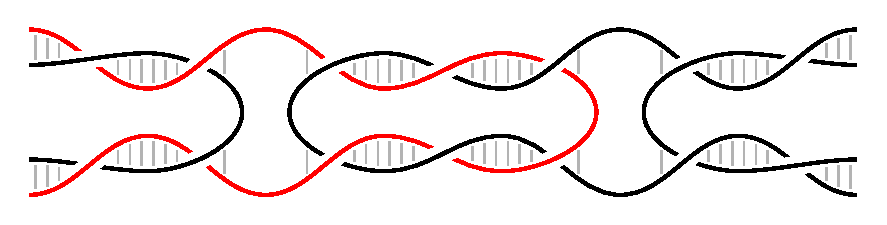
\includegraphics[width=\textwidth]{./figures/dao-dae/dao.pdf}
				\caption{DAO.}
				\label{fig:dae}
			\end{subfigure}
			\caption{DAO vs. DAE.}
			\label{fig:dao-dae}
		\end{center}
		\end{figure}
		
		In a real computation we will need to read the bottom line's sequence in a row thus it is practically reasonable to use DAE molecules. Moreover we will require even number of half-turns between crossovers in adjacent molecules. This is well explained in \cite[p.37]{winfree_phd}.
		
		DAE molecules thus have many reasons to be the most promising % citovat tunu praktickejch článků
		thus Chapter \ref{chap:problems} will be dedicated espacially to models with these molecules.

\section{Wang-tile models}

\subsection{Definition}
	
	% Winfree pg 56
	
	We will rather define Wang tile models less formally because it will be clear what they mean and excessive formality could cause confusions.
	
	Wang tile is a square tile with one color (also index, glue) from a finite nonempty set $I$ on each its edge\footnote{Tiles keep orientation, they are {\em not} allowed to rotate nor reflect.}, let us denote (nonempty) set of all available tiles $T$. Wang tiling is a mapping ${\cal T}: (\Z^2) \rightarrow T$ with restrictions: neighboring tiles must have the same color on the adjacent edge and its domain is required to be (topologically) connected. Wang tiling ${\cal T}_2$ is called {\em reachable} from Wang tiling ${\cal T}_1$ iff ${\cal T}_1 \subseteq {\cal T}_2$. A tiling $\cal T$ is called {\em terminal} iff there does not exist any strictly larger tiling reachable from $\cal T$. %!% říct jaký to uspořádání je, že má minimální prvek
	
	Winfree extends this definition for DNA tile assembly purposes and introduces Abstract Tile Assembly Model\footnote{Another model introduced by Winfree is Kinetic Tile Assembly Model ($\ktam$) which describes system dynamics.} ($\atam$). Additionally
	\begin{itemize}
		\item every color $c$ is associated with a nonnegative integer $g(c)$ which will also be referred to as {\em glue strength},
		\item there exists an empty color denoted by $\epsilon$ which can be neighboring with arbitrary color,
		\item tiling is only allowed to grow
		\begin{itemize}
			\item from a special initial tile denoted by $t_0$ from $(0,0)$ ({\em initial configuration}),
			\item one tile per step,
			\item the sum of glues connected in one step must be greater than or equal to given integer treshold\footnote{Interesting to study are small numbers like $1$, $2$; there are different results in Section \ref{sec:wang_power}}, so called {\em temperature}, denoted by $\tau$.
		\end{itemize}
	\end{itemize}
	Reachability relation will be restricted accordingly to these rules, {\em reachable in (tilesystem) $T$} will mean reachable from initial configuration, same for {\em terminal tiling in (tilesystem) $T$}.
	
	Similarly to Turing machines, tilesystem $T$ will be called:
	\begin{description}
		\item[Deterministic.] Iff there exists unique terminal tiling in $T$. % (in other words, reachability relation has one minimal/maximal member).
		\item[Non-deterministic.] Iff it has no other restrictions. % no ...
		\item[Probabilistic.] Iff every possible step in every stage has defined probability. See Note \ref{note:tilesystems} for our proposal how the probability could be defined.
	\end{description}
	
	\begin{note}\label{note:tilesystems}
		If there is a unique place and a unique tile the probability is $1$. If there is a unique place but there are more candidate tiles, the probability $\prob_C(t)$ of connecting tile $t$ should be distributed to these tiles somehow according to their ratio of concentration (denoted by $\prob_0(t)$) and their total connectible glue strength (denoted by $G(t)$). Most straightforward is weighted average:
		\begin{equation*}
			\prob_C(t) = \frac{G(t)\cdot\prob_0(t)}{\sum\limits_{u\textnormal{ possible tile}}G(u)\cdot\prob_0(u)}
		\end{equation*}
		In the most general case there are more places, each having several candidates. The probability $\prob_C(t,i)$ of connecting tile $t$ on place $i$ can be defined as weighted average again, now with one more sum over all possible places:
		\begin{equation*}
			\prob_C(t,i) = \frac{G(t,i)\cdot\prob_0(t)}{\sum\limits_{j\textnormal{ possible place}}\quad\sum\limits_{u\textnormal{ possible tile}\atop\textnormal{on place }j}G(u,j)\cdot\prob_0(u)}
		\end{equation*}
	\end{note}

% tady začíná moje práce => vyzdvihnout?

\subsection{Studied complexities}
	
	\begin{defn}
		\label{def:stud_compl}
		All the following complexities are considered as functions of size of the problem, which will be denoted by $n$:
		\begin{description}
			\item[Biostep complexity.] Refers to the number of laboratory steps required to handle the computation, denoted by $Bs(n)$. Adleman \cite{adleman95biostep} describes formally in his {\em unrestricted model} few types of such lab procedures -- {\em Separate, Merge, Detect} and {\em Amplify}, Winfree \cite{winfree_phd} adds another -- {\em Append}. Both of them remind that one biostep takes tens of minutes. Thus the only practically feasible DNA algorithms are those with $O(1)$ biostep complexity.
			\item[Binding complexity.] Refers to the number of bindings in terminal tiling\footnote{In deterministic computation the value is unique, in non-deterministic computation we consider the value for the smallest accepting terminal tile, in probabilistic computation we consider largest value due to the randomness.}, denoted by $Bnd(n)$. Too high binding complexity leads to lower probability of correct computation $P_c$ because it holds $P_c(n) = (1-p_e)^{Bnd(n)} \approx\footnote{If reasonable.} \; 1-p_e \cdot Bnd(n)$ where $p_e$ denotes probability of erroneous binding.
			\item[Tile complexity.] Refers to the number of different DNA tiles, denoted by $Ti(n)$. The higher tile complexity the more demanding it is to prepare required tiles.
			\item[Glue complexity.] Refers to the number of different sticky-end sequences (commonly referred to as {\em glues}), denoted by $Gl(n)$. Each sequence with its Watson-Crick complement is considered as one glue. Higher glue complexity will require longer DNA sequences in the sticky ends. % which leads to higher probability of erroneous binding $p_e$. %!% něco citovat co zminuje závislost p_e na dýlce sekvence, to přece musí rost ...
		\end{description}
	\end{defn}
	
	\begin{lemma}
	\label{lem:ti_gl}
		~
		\begin{enumerate}
			\item $Ti(n) \leq Gl^4(n)$,
			\item $Gl(n) \leq 4\,Ti(n)$.
		\end{enumerate}
	\end{lemma}
	\begin{proof}
		For combinatoric reasons,
		\begin{enumerate}
			\item having $Gl(n)$ glues, we cannot make more than $Gl^4(n)$ different tiles,
			\item having $Ti(n)$ tiles, there can appear maximally $4\,Ti(n)$ glues.
		\end{enumerate}
	\end{proof}
	
	\begin{thesis}
	\label{ths:feasible}
		Feasible DNA algorithms comply $Bs(n)\in O(1)$; $Bnd(n),\,Ti(n),\,Gl(n)\in \P$.
	\end{thesis}

% tahle subsection neni moje práce, zbytek už zase je

\subsection{Computational power}\label{sec:wang_power}
	
	The most exciting thing about $\atam$ is that
	\begin{itemize}
		\item it is known to be capable of universal computation at temperature $2$ in 2D,
		\item also at temperature $1$ in 3D,
		\item but it is not known to be universal or not at temperature $1$ in 2D\footnote{Universality has been reached only with modifications to the original model, see \cite{stage_assembly}, \cite{active_tiles}.}.
	\end{itemize}
	Let us show known results in the following table.
	
	\begin{center}
	\begin{tabular}{|| c || c | c | c ||}
		\hline\hline
		~ & \multicolumn{2}{c|}{\bf $n\times n$ squares} & {\bf Computational} \\
		~ & \multicolumn{1}{c}{LB} & \multicolumn{1}{c|}{UB} & {\bf Power}\\
		\hline
		$\tau=2$, 2D & \multicolumn{2}{c|}{See \cite{square_lb}, $\Theta(\frac{\log n}{\log\log n})$, see \cite{square_ub}} & Universal, see \cite{winfree_phd} \\
		\hline
		$\tau=1$, 3D & $\Omega(\frac{\log n}{\log\log n})$, see \cite{square_lb} & $O(\log n)$, see \cite{cook_temp1} & Universal, see \cite{cook_temp1} \\
		\hline
		$\tau=1$, 2D & $\Omega(\frac{\log n}{\log\log n})$, see \cite{square_lb} & $2n-1$, see \cite{square_lb} & Unknown \\
		\hline\hline
	\end{tabular}
	\end{center}

% tady pokračuje moje práce

\subsection{Turing universality of 2D tiles at $\tau=2$}
	
	Here we propose an alternative and more straightforward 2D tilesystem denoted by ${\cal T}_{TM}$ which directly simulates Turing machine at $\tau=2$ proving Turing universality of this model, see Figures \ref{fig:tileset1} and \ref{fig:tileset2}. All tiles are described within figures.
	\begin{remark}
		This tilesystem can simulate deterministic Turing machine as well as non-deter\-ministic or probabilistic if we consider corresponding tilesystem, all in $O(1)$ biosteps.
	\end{remark}
	The worst case occurs when the head is changing its step direction because all the rest of the tape must be copied. Following lemma gives upper bound for binding complexity as well as for the other studied complexities.
	\begin{lemma}
	\label{lem:TM_bound}
		Studied complexities in tilesystem ${\cal T}_{TM}$ are bounded as follows:
		\begin{description}
			\item[Biostep.] $Bs(n) \in O(1)$.
			\item[Binding.] $Bnd(n) \in O(t^2(n))$ where $t(n)$ denotes running time of the simulated Turing machine.
			\item[Tile.] $Ti(n) \in O(n)$.
			\item[Glue.] $Gl(n) \in O(n)$.
		\end{description}
	\end{lemma}
	\begin{proof}
		~
		\begin{description}
			\item[Biostep.] All tiles are designed to operate altogether thus only constant number of biosteps is needed.
			\item[Binding.] All Turing machine steps are simulated one-to-one or one-to-constant number of bindings with only one exception which is tape-copying as soon as head changes its direction. The length of %!% popsaný
			used tape is less than or equal to $t(n)$. Every copied length is thus bounded by $t(n) + C$ where $C$ is a constant, copying process is thus bounded by $2(t(n)+C)$ bindings. Copying occurs maximally once per simulated step thus number of copying is bounded by $t(n)$. Altogether number of bindings is bounded by $2(t(n)+C)\cdot t(n) \in O(t^2(n))$.
			\item[Tile.] Number of non-input tiles is constant, it is proportional to Turing machine size which is constant. There must only be prepared $n$ special input tiles thus $Ti(n) \in O(n)$.
			\item[Glue.] Follows from Lemma \ref{lem:ti_gl} which states that $Gl(n) \leq 4Ti(n)$.
		\end{description}
	\end{proof}
	\begin{cor}
	\label{cor:poly_resist}
		% in corresponding type of the model, i.e. determ, non-determ, prob
		
		In 2D at temperature $\tau = 2$ using corresponding type of $\atam$ (i.e. deterministic, non-deterministic or probabilistic), all classes resistant to polynomial slowdown ($\P$, $\ZPP$, $\RP$, $\BPP$, $\NP$, \ldots) remain preserved for all studied complexities. Moreover, biostep complexity remains in $O(1)$.
	\end{cor}
	
	\begin{figure}[h]
	\begin{center}
		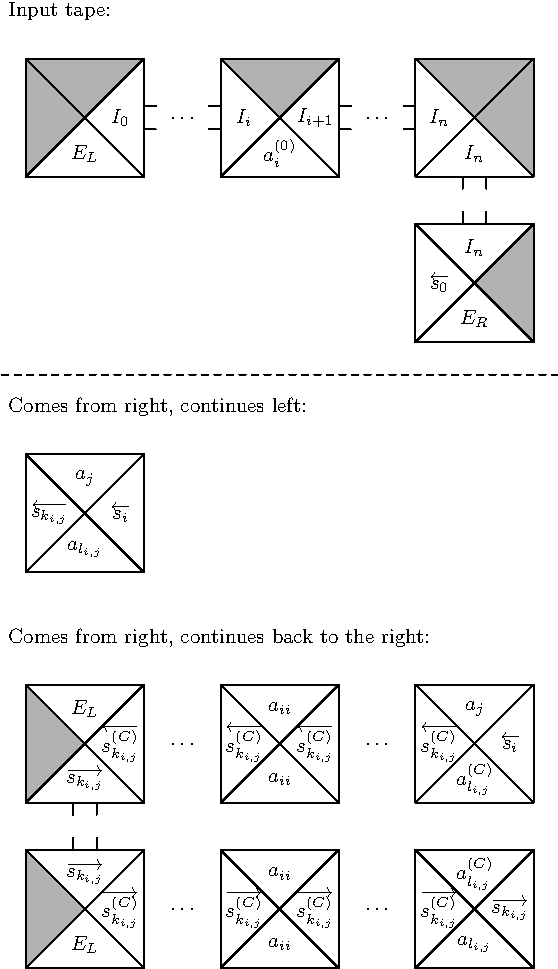
\includegraphics{./figures/tiles1.pdf}
		\caption{Tileset 1/2. Symmetric tiles are considered.}
		\label{fig:tileset1}
	\end{center}
	\end{figure}
	
	\begin{figure}[h]
	\begin{center}
		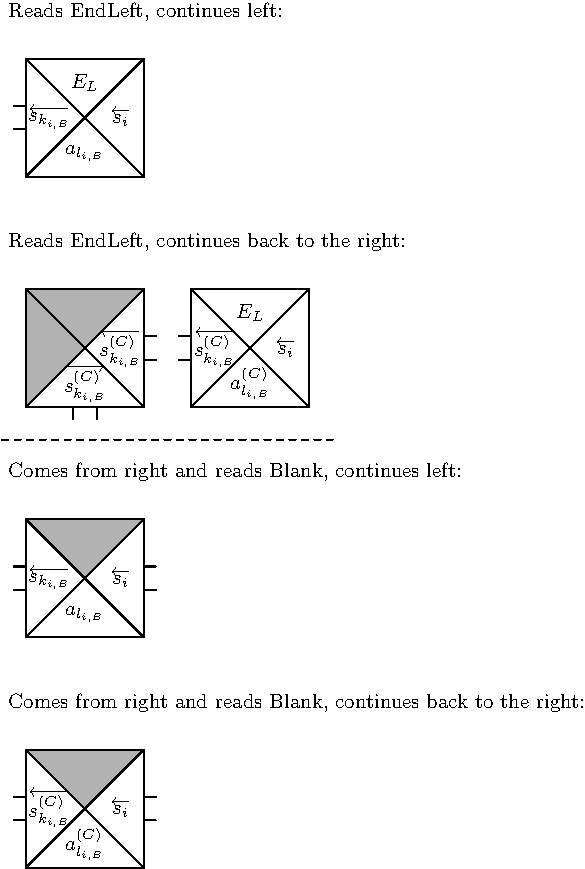
\includegraphics{./figures/tiles2.pdf}
		\caption{Tileset 2/2. Symmetric tiles are considered.}
		\label{fig:tileset2}
	\end{center}
	\end{figure}

\subsection{Feasibility of the class $\BPP$}
	
	Remind that every language from $\BPP$ is decidable on a PTM in polynomial time which means that probability of correct result is greater than $\nicefrac{2}{3}$. Note that one can reach probability of correct result higher than arbitrary constant smaller than $1$ by constant number of iterations. Thus it is reasonable to consider $\BPP$ as practically feasible.   % \footnote{Considering even Quantum Turing machine to be practically feasible, $\BQP$ (a superset of $\BPP$) would be practically feasible. Note that due to Shor's algorithm \cite{shor94}, Integer Factorization Problem belongs to $\BQP$ but it is assumed that it does not belong to $\BPP$. Thus $\BPP$ is assumed to be proper subset of $\BQP$.}
	
	Here we introduce a similar proposal for feasibility of DNA algorithms. In Definition \ref{def:stud_compl} we proposed that biostep complexity of feasible algorithms must comply $Bs(n)\in O(1)$ which is proved in Lemma \ref{lem:TM_bound} for Turing universal tilesystem ${\cal T}_{TM}$. In Thesis \ref{ths:feasible} we proposed that other studied complexities must be polynomial and Corollary \ref{cor:poly_resist} states preserving of classes $\P$, $\ZPP$, $\RP$, $\BPP$, $\NP$, \ldots ~in tilesystem ${\cal T}_{TM}$ at temperature $\tau=2$. Note \ref{note:tilesystems} proposes how a probabilistic $\atam$ could be practically simulated. These arguments altogether justify Corollary \ref{cor:bpp_feas}.   %!% přečíst po sobě
	
	\begin{cor}
	\label{cor:bpp_feas}
		$\BPP$ is feasible in 2D at temperature $\tau=2$.
	\end{cor}
	
	\begin{note}
		Remind that $\P$, $\ZPP$, $\RP$ and $\coRP \subseteq \BPP$.
	\end{note}
	
	
	
	%!% popsat co znamená že je něco sestavitelný -- NP, že má něco pst sestavení -- BPP
	
	%%%%%%%%%%%%%%%%%%%%%%%%%%%%%%%%%%%%%%%%%%%%%%%%%%%%%%%%%%%%%%%%%%%%%%
	
	% error-tolerant rules -- Gacs and Reif, 1988\\



%%% KAPITOLA 2
\chapter{Strand models}

% úvod o kapitole, přehled

Quick overview of considered structures. Winfree's overview (pg 29 -- considered molecules, pg 36 -- sizes of DAE and a better picture, pg 37 -- comparison of DAO/DAE in a lattice, explanation pg 43).

Seeman, Fu and their DAO/DAE in \cite{seeman93}, is the picture of DAO strange?

\section{Adleman's experiment}
	
	Adleman showed in his ground-breaking work, \cite{adleman94}, that DNA molecules are really capable of computation. He exploited that huge parallelism possible in DNA computation for one of the most fundamental NP-complete problems -- the Hamiltonian Path Problem (HPP) in directed graph with designated vertices $v_{begin}$ and $v_{end}$.
	
	Let us remind this type of HPP. Given a directed graph $G_n$ with $n$ vertices and two designated vertices $v_{begin}$ and $v_{end}$, the problem is to answer whether there exists an oriented path from $v_{begin}$ to $v_{end}$ through the graph such that the path visits every vertex. Note that {\em path} cannot visit any vertex more than once from definition.
	
	\begin{figure}[H]
	\begin{center}
		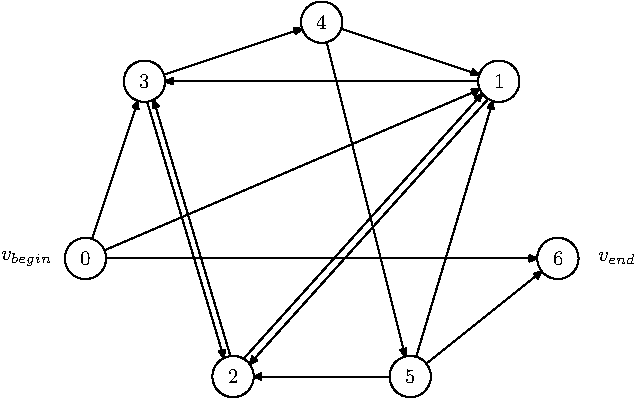
\includegraphics{./figures/adleman_graph.pdf}
		\caption{Adleman's original graph.}
		\label{fig:adleman_graph}
	\end{center}
	\end{figure}
	
	Adleman originally used a graph with seven vertices shown in figure \ref{fig:adleman_graph}. It can be seen that the path $0 \rightarrow 1 \rightarrow 2 \rightarrow 3 \rightarrow 4 \rightarrow 5 \rightarrow 6$ is Hamiltonian\footnote{Note that it can be re-labelled such a nice way without loss of generality.}.
	
	Adleman first presents this non-deterministic five-step algorithm, whose steps are then described in terms of DNA manipulations:
	\begin{description}
		\item[Step 1] Generate random paths through the graph.
		\item[Step 2] Keep only those paths that begin with $v_{begin}$ and end with $v_{end}$.
		\item[Step 3] If the graph has $n$ vertices, then keep only those paths that enter exactly $n$ vertices.
		\item[Step 4] Keep only those paths that enter all of the vertices of the graph at least once.
		\item[Step 5] If any paths remain, say ``Yes''; otherwise, say ``No.''\footnote{This is the original version, I would rectify the fifth step: If any paths remain, say ``Yes''; otherwise, say ``{\em I do not know.}'' That is because NP problem gives answer ``Yes'' iff there {\em exists} supporting solution. To say ``No'' one needs to show that {\em all} solutions do not satisfy. That is exactly the difference between NP and co-NP.}
	\end{description}
	To see % sloveso od insight ?
	how DNA can compute, let us describe this example more precisely. The computation itself (I mean the inception of the final solution) is hidden in Step 1. Each vertex $i$ is associated with a random\footnote{We will expect those sequences to be different enough.} $20$-mer sequence of DNA, let us denote its $5'\rightarrow 3'$ orientation by $O_i$, its 10-mer prefix by $p_i$ and its 10-mer suffix by $q_i$. Each edge $i\rightarrow j$ is then associated with $\overline{q_i p_j}$ sequence with reverse backbone orientation ($3'\rightarrow 5'$) where $\overline{q_i}$ stands for Watson-Crick complementary word. There is an exception for $i=begin$ and $j=end$: instead of $\overline{q_{begin} p_j}$ there is $\overline{O_{begin} p_j}$ and in a similar way for $j=end$.
	
	\begin{figure}[H]
	\begin{center}
		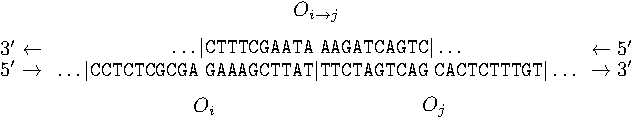
\includegraphics{./figures/adleman_strands.pdf}
		\caption{Example of assigned sequences.}
		\label{fig:adleman_strands}
	\end{center}
	\end{figure}
	
	It can be easily seen that all correctly bonded double-strands correspond with a valid path in $G_n$. Moreover, all complete double-strands represent a valid path from $v_{begin}$ to $v_{end}$ through $G_n$.
	
	All the other steps are fully described in \cite{adleman94}. The most important thing is that the most time-demanding step is Step 4. In this step one has to purify the product of Step 3 with a biotin-avidin magnetic beads system. This process extracts consequently for every vertex $i$ only those DNA strands which contain a substring representing vertex $i$. Thus its biostep complexity is $O(n)$. If we assume that one biostep takes at least tens of minutes and it should be performed repeatedly to avoid errors, we can conclude that $O(n)$ is just too much\footnote{Winfree, \cite{winfree_phd}, gives a positive solution.}.

\section{Single-stranded molecules}
	
	SAT in $O(1)$ biosteps etc.

\section{Double-stranded molecules}
	
	\subsection{Linear strands}
		
		Equivalent to regular languages.
	
	\subsection{Dendrimer structures}
		
		Equivalent to context-free languages.

\section{Double crossover molecules}
	
	Equivalent to recursively enumerable languages (Turing universal). Important notes in 3.2.5 Winfree -- single side hybridization -- how to avoid. Tricky solution of Hamiltonian Path Problem.

%%% KAPITOLA 3
\chapter{Wang tile models}   % Hasentiles! Hase = zajíc (D)

\section{Definition}
	
	More abstract model where one handles only with ``glues'' on edges of Wang tiles. Define {\em temperature}.

\section{Computational power}
	
	Give table of Turing universality \cite{cook_temp1}.
	
	See \cite{winfree_phd}. Many other results in \cite{cook_temp1}, \cite{stage_assembly}, \cite{square_lb}, \cite{square_ub} \ldots
	
	\subsection{Turing universality of 2D tiles at $T=2$}
		
		\begin{figure}[H]
		\begin{center}
			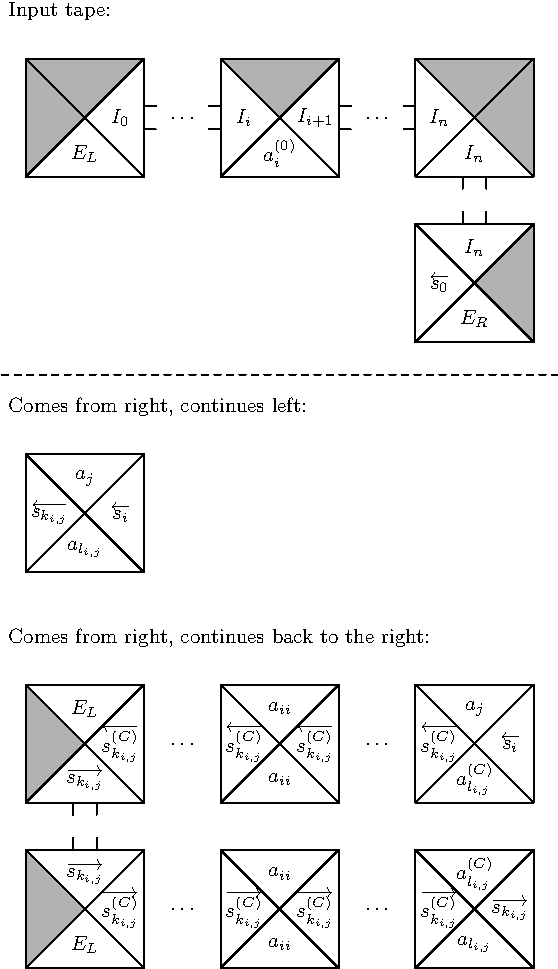
\includegraphics{./figures/tiles1.pdf}
			\caption{Tileset 1/2.}
		\end{center}
		\end{figure}
		
		\begin{figure}[H]
		\begin{center}
			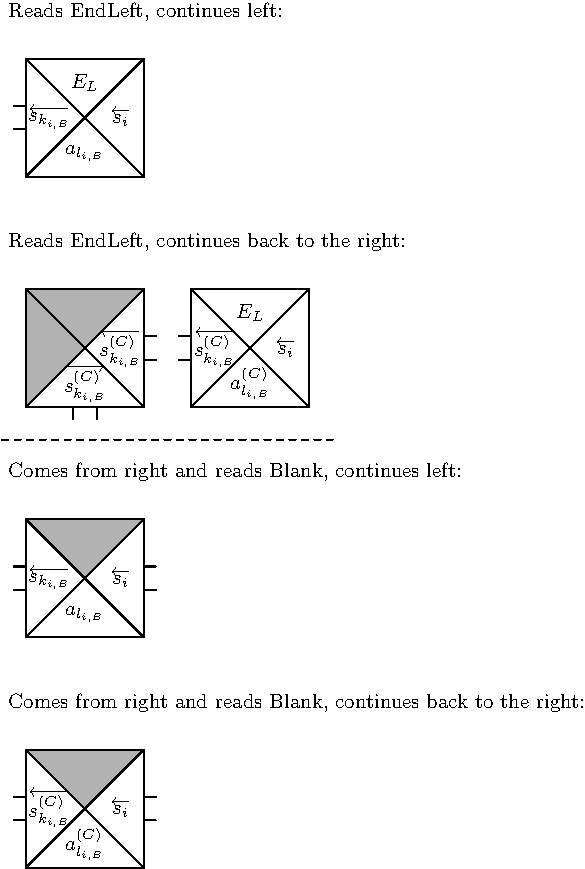
\includegraphics{./figures/tiles2.pdf}
			\caption{Tileset 2/2.}
		\end{center}
		\end{figure}
	
	%%%%%%%%%%%%%%%%%%%%%%%%%%%%%%%%%%%%%%%%%%%%%%%%%%%%%%%%%%%%%%%%%%%%%%
	
	error-tolerant rules -- Gacs and Reif, 1988\\


%%% KAPITOLA 4
\chapter{Results}

\section{Abstract model for DAE units}

% \section{Abstract model for DAE units}

It is better to draw easier-to-understand pictures. Explanation: \ldots Call those DNA sequences ``glues''.

In following examples this model will be set up to act similarly like NP: $\exists y \; R(x,y)$. Although existence is not sure, it is very likely. Predicate $R$ will be ``enumerable in polynomial time'' for $x \in L$. In this context, {\em enumerable in polynomial time} will mean number of bindings, not number of biosteps. This can be assumed due to Turing universality of this model in $O(1)$ biosteps -- biostep complexity is not restrictive\footnote{From Turing's thesis, Turing machine is the most universal model.} and will be required to be $O(1)$ due to its lab complexity. On the other hand the binding complexity will be very important, we will be interested even in constants. This is because the less binding complexity, the less probability of error.

% diskutovat pravděpodobnost objevení vs. neobjevení $y$ !!! dát odkaz do footnote
% odhady se dají zmenšit pomocí #E místo #V^2

Define (slightly more correctly) binding complexity of this model as the number of bindings. Only the biggest term will be considered but even with constant.

\begin{figure}[h]
\begin{center}
	\begin{subfigure}[b]{0.31\textwidth}
		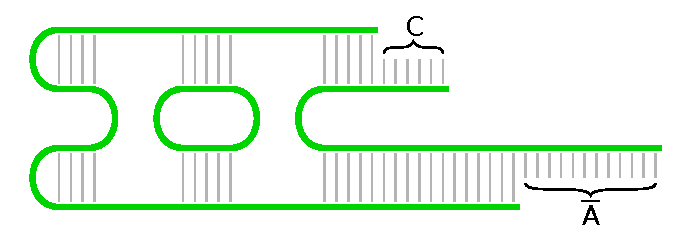
\includegraphics[width=\textwidth]{./figures/tile_model/DNA_struct.pdf} % 115mm
		\caption{Corner DAE unit}
		\label{fig:DNA_struct}
	\end{subfigure}%
	%add desired spacing between images, e. g. ~, \quad, \qquad etc.
	%(or a blank line to force the subfigure onto a new line)
	\begin{subfigure}[b]{0.472\textwidth}
		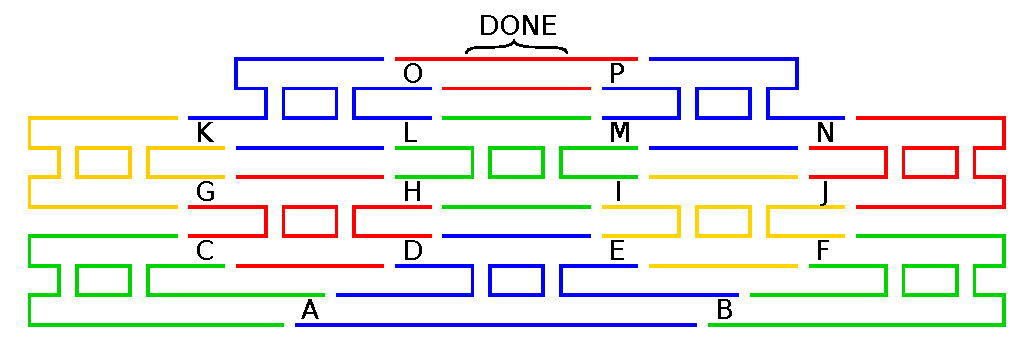
\includegraphics[width=\textwidth]{./figures/tile_model/DNA_assembly.pdf} % 175mm
		\caption{Whole self-assembly}
		\label{fig:DNA_assembly}
	\end{subfigure}
	\begin{subfigure}[b]{0.190\textwidth}
		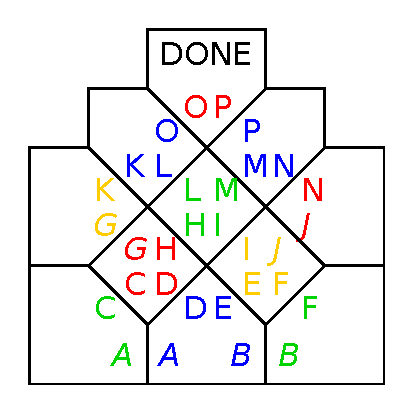
\includegraphics[width=\textwidth]{./figures/tile_model/abstract_model.pdf} % 70mm
		\caption{Abstract model}
		\label{fig:abstract_model}
	\end{subfigure}
	\caption{Evolution of abstract model from DAE units to tiles.}
	\label{fig:evolution}
\end{center}
\end{figure}



\section{Graph 3-coloring}

% \section{Graph 3-coloring}

Remind original Knuth's algorithm at \url{http://www.iti.fh-flensburg.de/lang/algorithmen/sortieren/networks/oetsen.htm}! And prove that everything goes fine!

First idea: Generate all bonds with colored atoms and check the entire system (haha, complexity like $O(n^4)$ because $|E| \in O(n^2) $). Second solution: Generate a reverse-order sequence of vertices and let it order in the correct order. All pairs should meet each other, the problem to solve is whether all pairs really meet each other. After that check that the area is full like Winfree -- from one side to the other. Improvement: the check can be triggered from both sides simultaneously.

The first idea was like $O(n^4)$, the second one is already $O(n^2)$, the binding complexity is $1\nicefrac{1}{2}\;n^2$. The improvement decreases it to $1\nicefrac{1}{4}\;n^2$.

\subsection*{Set of tiles}

First of all the graph needs to have even number of vertices, thus one separated non-colored vertex has to be added if applicable. Then follow these rules which are showed in an example, see figure \ref{fig:3-color}.
\begin{description}
	\item[Bottom line] For every pair $(2k,\,2k+1)$ there will be a bottom-type tile with non-colored numbers $(2k+2,\,2k)$ on the bottom and with all feasible\footnote{If $(2k+1,\,2k)$ are connected, same-colored numbers are omitted.} color combinations of $(2k+1,\,2k)$ on the top. From practical decoding reasons (see Winfree \cite{winfree_phd}) the sequences encoding colored numbers on the top must be physically present also wherever on the bottom DNA strand, see figure \ref{fig:bottom_tile}. $\frac{9n}{2}$ tile types were required.
	\item[Bottom corner tiles] Both corner tiles are connected on the bottom by the highest and the lowest non-colored number, respectively, and have their special glue (\# for $-\infty$ and * for $+\infty$, respectively) on the top. These first two sets of tiles generate all colorings of given graph (without those omitted in previous step) with reverse order of numbers. $2$ tile types were required.
	\item[Inner tiles] These tiles are responsible for ordering\footnote{Principially they are the same as in Winfree \cite{winfree_phd}.}. There exist all color combinations for all different numbers with two important exceptions. There {\em do not} exist tiles with numbers of connected vertices with the same color. Thus, as soon as there appears such forbidden combination, the self assembly cannot continue and reach ``DONE''. Because the numbers are generated in reverse order they must meet each other -- note that they simply cannot ``jump'' and every number has to exchange with all the higher ones as well as with the lower ones. This implies that every forbidden combination would be revealed, thus it answers correctly if and only if the coloring is correct. The second exception are those described in the following paragraph. $9n^2$ tile types were required.
	\item[Border tiles] There are two tile types on the borders, one with sharp, one with asterisk. They keep the structure growing up.
	\item[Checking tiles] As soon as the biggest and the smallest number reach * and \#, respectively, there are two special tiles which start checking whether nothing is missing. Note that all tiles had time enough to get into correct order. In this setup checking tiles do not need to check correct order thus there can exist only two types of checking sequences ``C'' and ``D'' with all color-number combinations of middle numbers -- ``D'' with the smaller half, ``C'' with the higher half. $3n$ tile types were required.
	\item[DONE tile] If everything is checked and checking sequences meet each other, ``DONE'' tile will be connected to signalize correct solution. $1$ tile type was required.
\end{description}
\begin{figure}[H]
\begin{center}
	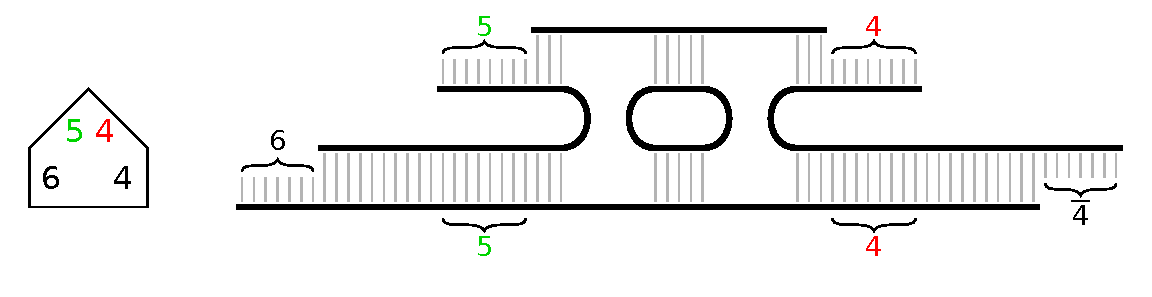
\includegraphics[scale=0.75]{./figures/3-color/bottom_tile.pdf}
	\caption{Bottom tile with desired sequences in the bottom strand.}
	\label{fig:bottom_tile}
\end{center}
\end{figure}
Summed up, this DNA algorithm requires $9n^2$ tile types.

\begin{figure}[H]
\begin{center}
	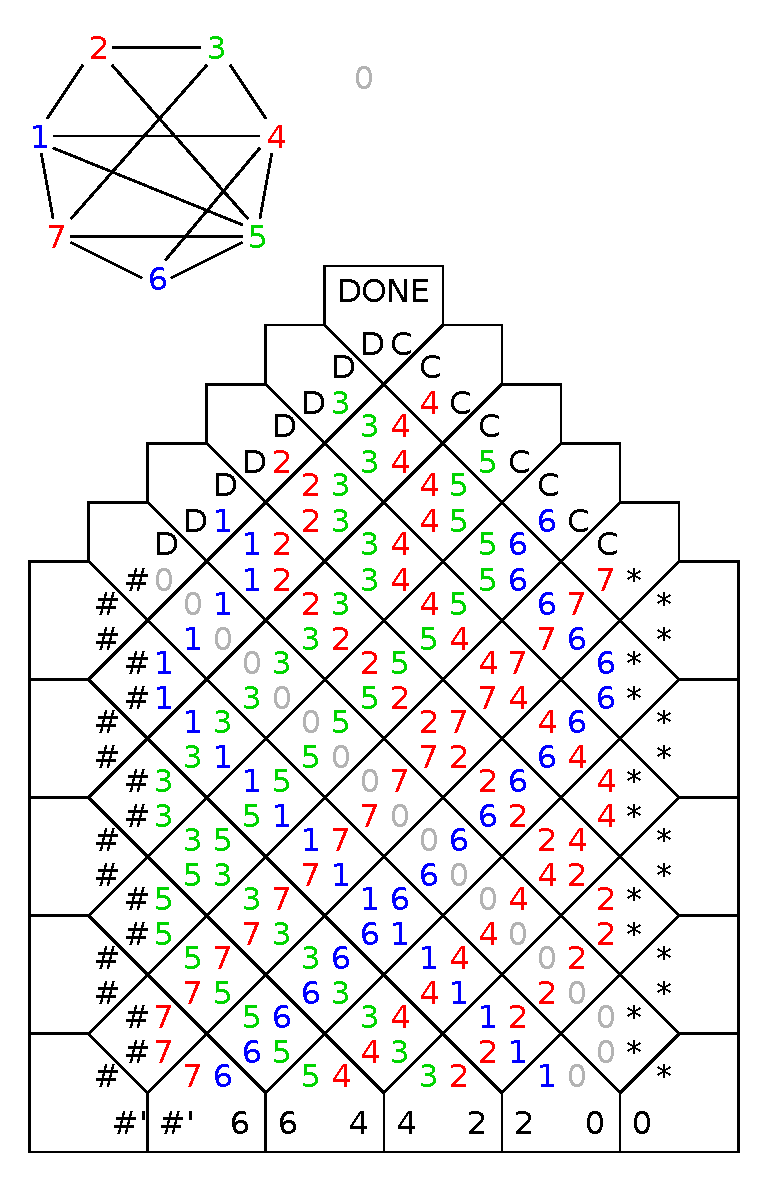
\includegraphics[scale=0.75]{./figures/3-color/3-color.pdf}
	\caption{3-color computation.}
	\label{fig:3-color}
\end{center}
\end{figure}



\newpage
\section{Graph isomorphism}

% \section{Graph isomorphism}

Graph isomorphism problem clearly belongs to NP but it does not seem to be NP-hard\footnote{Clearly, if P = NP it would even belong to P.} \cite{borec_z_wiki}. Thus it seems that it is neither P nor NP-complete. From this reason it seems to belong to a special class and thus I will describe a DNA system which solves this very special problem. % vocitovat

Surprisingly it is very similar to 3-coloring if we consider $n$ colors instead. The problem can be stated: ``For a non-colored graph $G$ and a graph $H$ where every vertex is colored with different color, find a coloring of $G$ with all of those $n$ colors used exactly once (1) such that these colored graphs are isomorphic (2).'' Now one has to check that:
\begin{enumerate}
	\item every ``color'' was used exactly once so that it is a bijection,
	\item edges and non-edges are preserved.
\end{enumerate}

\subsection*{Set of tiles}

Like before, the graph needs to have even number of vertices, thus one separated self-bijective vertex has to be added if applicable. An example is given, see figure \ref{fig:graph_iso}.
\begin{description}
	\item[Bottom line] These tiles have almost exactly the same rules as in graph 3-coloring, the difference is that {\em all} of the same-colored combinations are omitted. $\frac{n^3}{2}$ tile types were required.
	\item[Bottom corner tiles] Are exactly the same. $2$ tile types were required.
	\item[Inner tiles] There are three types of inner tiles:
	\begin{description}
		\item[Number-ordering tiles] These are similar to previous ones, the difference is which do exist and which do not. Let us assume a tile with numbers $k$ and $l$ with colors $a$ and $b$, respectively. Note that numbers $k$ and $l$ correspond with vertices in graph $G$ and colors $a$ and $b$ correspond with vertices in graph $H$. This tile must check the isomorphism property -- existence or non-existence of edge between appropriate vertices. Thus the tile exists if and only if
		$$(\{k,\,l\} \in E(G) \wedge \{a,\,b\} \in E(H)) \vee (\{k,\,l\} \notin E(G) \wedge \{a,\,b\} \notin E(H)) . $$
		From similar reasons all pairs of vertices from graph $G$ meet each other, thus every edge is checked so condition number $2$ would be done. $n^4$ tile types were required.
		\item[Color extracting tiles] Now I have to extract colors (forget numbers) and order them in given order so that I can check that every color is used exactly once. This process will be triggered by a special inner tile with the highest number of arbitrary color and a non-colored asterisk on the bottom. On the top it will have an asterisk of that number's color and a non-colored asterisk. For every other number with arbitrary color there exists a tile with it and an asterisk of an arbitrary but different color on the bottom. On the top it will have two asterisks of these colors in correct order. $n^3$ tile types were required.
		\item[Color-ordering tiles] These are similar to those with numbers. Similarly there do not exist tiles with one color. $n^2$ tile types were required.
		% there is some redundancy .. but no idea how to do it faster .. it can be done easier, one can only check without colors, same colors are killed during ordering!
	\end{description}
	\item[Border tiles] These tiles are exactly the same like for 3-coloring.
	\item[Checking tiles] As soon as there appears a combination of sharp and most-left-colored asterisk, a checking tile comes having ``C'' of the second color on the right top. After this initialization there are tiles with colored ``C'' and same-colored asterisk on the bottom and next-colored ``C'' on the right top. This ensures that every color was used exactly once. The last color is followed by non-colored ``C''. $n$ tile types were required.
	\item[DONE tile] Finally if non-colored ``C'' meets non-colored asterisk, a ``DONE'' tile is connected signalizing correct solution. $1$ tile type was required.
\end{description}
Summed up, this DNA algorithm requires $n^4$ tile types.

% .. místo na trik

\begin{figure}[H]
\begin{center}
	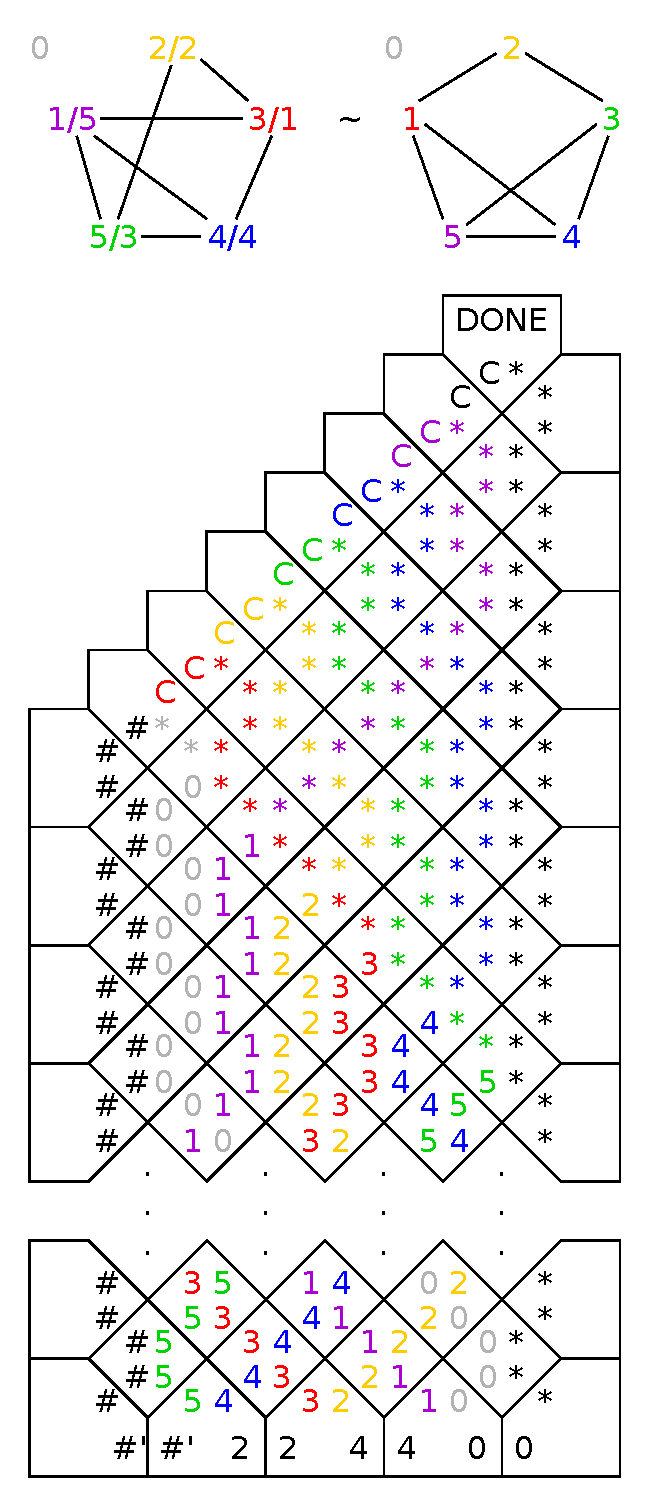
\includegraphics[scale=0.75]{./figures/isomorphism/isomorphism.pdf}
	\caption{Graph isomorphism computation. Color order is defined by their wavelength.}
	\label{fig:graph_iso}
\end{center}
\end{figure}



\newpage
\section{$k$-clique}

% \section{$k$-clique}

$k$-clique problem belongs to NP-complete problems. Note that $k$-clique problem in $G$ is equivalent to $n-k$ independent set in $\overline{G}$ so we can assume $k \leq \frac{n}{2}$. Like before we add an unchecked vertex if $k$ is odd so we will assume $k$ to be even. % možná: and there exists a DNA system with very low complexity: $\min\bigl\{ 1\nicefrac{1}{4}\;\bigl( \frac{n}{2} \bigr) ^2 ,\; 1\nicefrac{1}{4}\;k^2 \bigr\}$.

\subsection*{Set of tiles}

\begin{description}
	\item[Bottom line] For now there are tiles with $2l-2$ and $2l$ ($0 < l \leq \frac{k}{2}$) on the bottom and with an arbitraty ordered\footnote{Note that this restriction does not reduce the set of possible $k$-member subsets.} pair of different numbers from $1$ to $n$ with $k-2l+2$-th and $k-2l+1$-th colors, respectively, on the top. Note that now the order of colors is given and do not forget that they should also contain those upper sequences once more on the bottom strand. $\frac{kn^2}{4}$ tile types were required. % na prvních místech nejnižší čísla, na nejvyšších ty nejvyšší -> sníží počet dlaždic ale je s tim sraního
	\item[Bottom corner tiles] Are exactly the same. $2$ tile types were required.
	\item[Inner tiles] These tiles are now responsible for ordering by color during which they check existence of {\em every} edge in similar manner to previous problems. And because the first line contains them in reverse order there will meet each other. $k^2 n^2$ tile types were required. % $k^2 \cdot 2#E $
	\item[Border tiles] These tiles are exactly the same like for 3-coloring.
	\item[Checking tiles] As soon as the most left color reaches sharp and the most right color reaches asterisk, checking is triggered in similar manner to 3-coloring. $kn$ tile types were required.
	\item[DONE tile] This is exactly the same like 3-coloring. $1$ tile type was required.
\end{description}
Summed up, this DNA algorithm requires $k^2 n^2$ tile types. % $k^2 \cdot 2#E $

\begin{figure}[H]
\begin{center}
	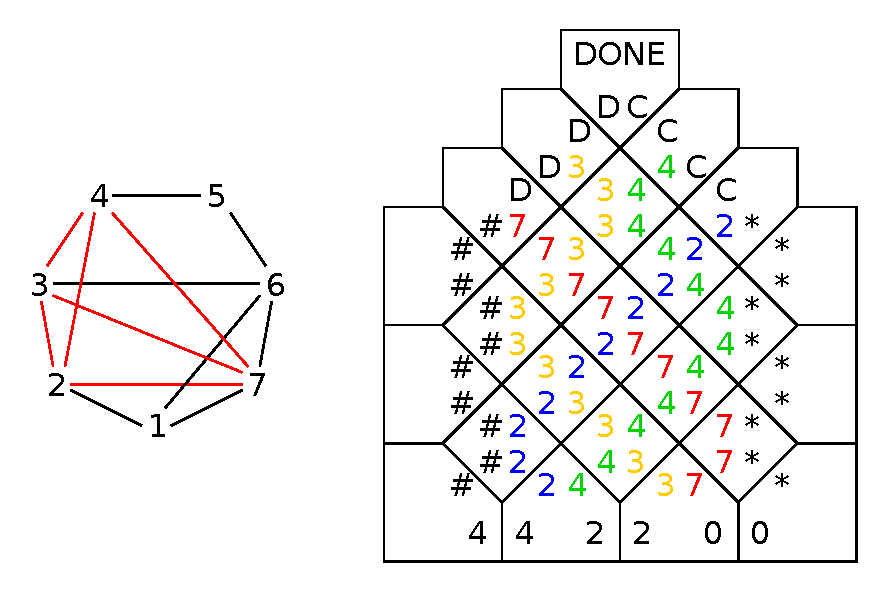
\includegraphics[scale=0.75]{./figures/k-clique/k-clique.pdf}
	\caption{$k$-clique computation. Color order is defined by their wavelength.}
	\label{fig:graph_iso}
\end{center}
\end{figure}




%%% ZÁVĚREM
\cleardoublepage\phantomsection   % cleardoublepage a phantomsection udělají že odkaz z obsahu vede NAD nadpis, jinak vede POD
\addcontentsline{toc}{chapter}{Epilog}
\chapter*{Epilog}
	
	The very last section to be done.

%%% LITERATURA
% \renewcommand\bibname{Literatura}
\cleardoublepage\phantomsection   % cleardoublepage a phantomsection udělají že odkaz z obsahu vede NAD nadpis, jinak vede POD
\addcontentsline{toc}{chapter}{References}

\bibliography{biblio}{}
\bibliographystyle{plain}


%%%%%%%%%%%%%%%%%%%%%%%%%%%%%%%%%%%%%%%%%%%%%%%%%%%%%%%%%%%%%%%%%%%%%%%%
%     K O N E C   P R Á C E                                            %
%%%%%%%%%%%%%%%%%%%%%%%%%%%%%%%%%%%%%%%%%%%%%%%%%%%%%%%%%%%%%%%%%%%%%%%%


\end{document}